\section{A ``hand-wavy'' first approach}

What we refer to as Artificial Intelligence is a broad 
collection of methods and techniques used to solve a wide array 
of problems that we collectively associate with ``human 
intelligence'', such as identifying and classifying images, 
processing natural language, and learning from data.  Roughly 
speaking, the discipline can be divided in the following 
sub-fields of research:

\begin{itemize}
	\item Neural Networks.
	\item Vision.
	\item Natural Language Processing.
	\item Speech processing.
	\item Machine Learning.
\end{itemize}

This thesis is concerned specifically with Machine Learning.  
Particularly with a subset of Machine Learning known as 
unsupervised learning.  Some authors \cite{SuttonBarto} insist 
Reinforcement Learning is itself different from unsupervised 
learning, but for the sake of simplicity we address the 
distinctions later on.

In contrast to supervised learning where a learning agent is 
given data labeled by a knowledgeable source and must ``learn'' 
to classify based on those initial labels, in unsupervised 
learning there is no ``train data'', the agent must act and 
optimize it's strategy based only upon the reward or penalty 
resulting from making a certain decision.  The key words here 
being \textit{optimize}, \textit{strategy} and 
\textit{decision}.

For a concrete example, picture a robot vacuum cleaner tasked 
with moving from an initial point to a target point.  Only that 
this robot has no sense of direction, it can only move up, down, 
left or right with respect to itself. The robot cannot ``tell'' 
which way to go, it only senses if got closer or farther away. 
Is there a way the robot can reach it's goal?

If you think about it, the robot analogy is not so different 
from the standard mental model we have of say an infant learning 
to crawl.  With poor vision and only it's caretaker's voice as 
guide, it must learn to find its way to safety by trial and 
error. It cannot be given millions of examples of ``valid 
paths'' for extrapolation, as is the case with supervised 
learning. This agent learns by interacting with the environment 
itself.

In a certain sense, Reinforcement Learning leverages our 
intuitions about the nature of learning. All the main elements 
are there: cause and effect, goals, and consequences to 
decisions made, but as we will see, it also encodes more subtle 
concepts. For instance, delayed gratification and planning 
ahead. It also has the novelty of being goal-oriented rather 
than task-oriented as most Machine Learning techniques often 
are. For example, a self-driving car ``trained'' via supervised 
learning might train on millions of examples on what constitutes 
a valid steering wheel move, while one learning without 
supervision is learning how to drive as an activity consisting 
of hundreds of little tasks, all to be mastered.

\section{Formalizing ideas}
Now, mathematically speaking, what does it \textit{mean} for a 
machine to ``learn''?

We might not get as far as what learning as a whole means for 
humans or machines, but we can certainly discuss what mechanisms 
allow for things such as self-driving cars and computers beating 
world champions of Chess and Go. For that, we need to identify 
the key concepts in the picture I painted and express them in 
the language of mathematics.

For now, we can gloss over the details of how might a machine 
make decisions, perceive goals, take actions or perceive 
rewards. Let's focus on one key component: the ``learning''. 
When we talk about a machine learning something we are thinking 
about some agent that is able to keep track of the decisions it 
made before and whether or not they resulted in positive results 
so it can later on apply that knowledge to become an 
increasingly better problem solver. If this agent is scored each 
time it carries on some task, we would like for it's score to 
increase each successive time it tries to complete the task. The 
idea of a continually improving score is the foundation of 
mathematical optimization.

\subsection{Optimization Theory}
As the name suggests, mathematical optimization is concerned 
with finding the ``optimal'' solution to problems where an 
unambiguous score might be given to different solutions.  
Whatever ``optimal'' means. Even if there is no best solution to 
a given problem, the techniques used in mathematical 
optimization often allow for a continual improvement through 
iteration.

Going back to our example of a robot learning how to drive, each 
time this robot runs a particular course it receives a certain 
grade. For instance, crashing or going off the circuit result in 
a penalty (negative grade) and respecting traffic signals 
results in a reward.  If we want the robot to become an 
increasingly better driver we must frame the process of 
successive tries as an optimization problem. If we are able to 
solve this problem and achieve a continually improving grade, 
our robot will in a sense be learning to be a better driver.

We are now ready to peel away another layer of abstraction.  We 
now have an intuition of what it means for a machine to learn, 
or in other words continually improve. But in the model we 
discussed earlier, this robot is making choices along the way. A 
predefined path is not programmed or even known. What does it 
mean for this robot to ``make choices''?

\subsection{Stochasticity}
Another key aspect we take for granted when we talk about 
machines learning is implicit in the word leaning. If there were 
a predefined path for the robot to take we would hardly call 
that learning, it's merely reproducing instructions.  What this 
means for us, is that we must allow for a framework in which our 
robots actions are not completely determined beforehand. In 
fancier words, the succession of events that determine the 
robots actions and responses to stimuli are not 
\textit{deterministic}.

This idea is formalized through something called a 
\textit{stochastic process}. The word stochastic is just 
mathematician speak for ``not entirely determined beforehand'' 
or ``aptly described as a random phenomena''.  In particular, we 
can think of the robot as being in some state among many many 
possible. The robot can change states as time goes by but the 
transitions are not always the same and they don't always carry 
the same reward or punishment.

For instance, on a certain circuit speeding up is bad, while on 
others its appropriate. You wouldn't drive at the same speed on 
a street as you do on a highway, even if they are both straight 
paths.  If the robot were learning anything it would know this. 
In both cases its current state is ``driving down a straight 
path'', but transitions to a state of breaking or accelerating 
for both scenarios are not equally likely, nor they should be.

\section{Wrapping up}
So far we have developed a mental model of what to do should we 
wish to teach a robot how to drive. The rest of this thesis is 
dedicated to the careful development of the ideas here presented 
into the language of mathematics. But beyond mere description, 
this exercise has the potential to unlock \textit{insight}. As 
is often said by legendary math communicator Grant 
Sanderson\footnote{From the YouTube channel 
\href{https://www.youtube.com/channel/UCYO_jab_esuFRV4b17AJtAw}{3blue1brown}}(loose 
quote), the point in formulating things this way is to gain a 
deeper understanding of the phenomenon. So let's dive right in.

\begin{figure}
\centering
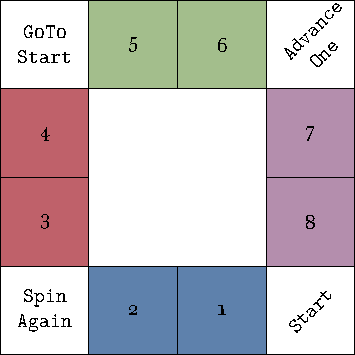
\includegraphics[width=0.5\textwidth]{img/board.pdf}
\caption{Board of a popular trademarked game}
\end{figure}
